\chapter{Experimental setup}

\section{Simulation environment}
\subsection{Table Clearing Environment}
In table clearing environment, main components are a 6 axis ABB IRB 120 robot with MetalWork W155032001 parallel jaw gripper and a table with yellow and green tray. Object at random position and orientation is inserted into the source tray (yellow). The task is to move the object from source tray (yellow) to destination tray (green).

\begin{figure}[H]
	\centering
	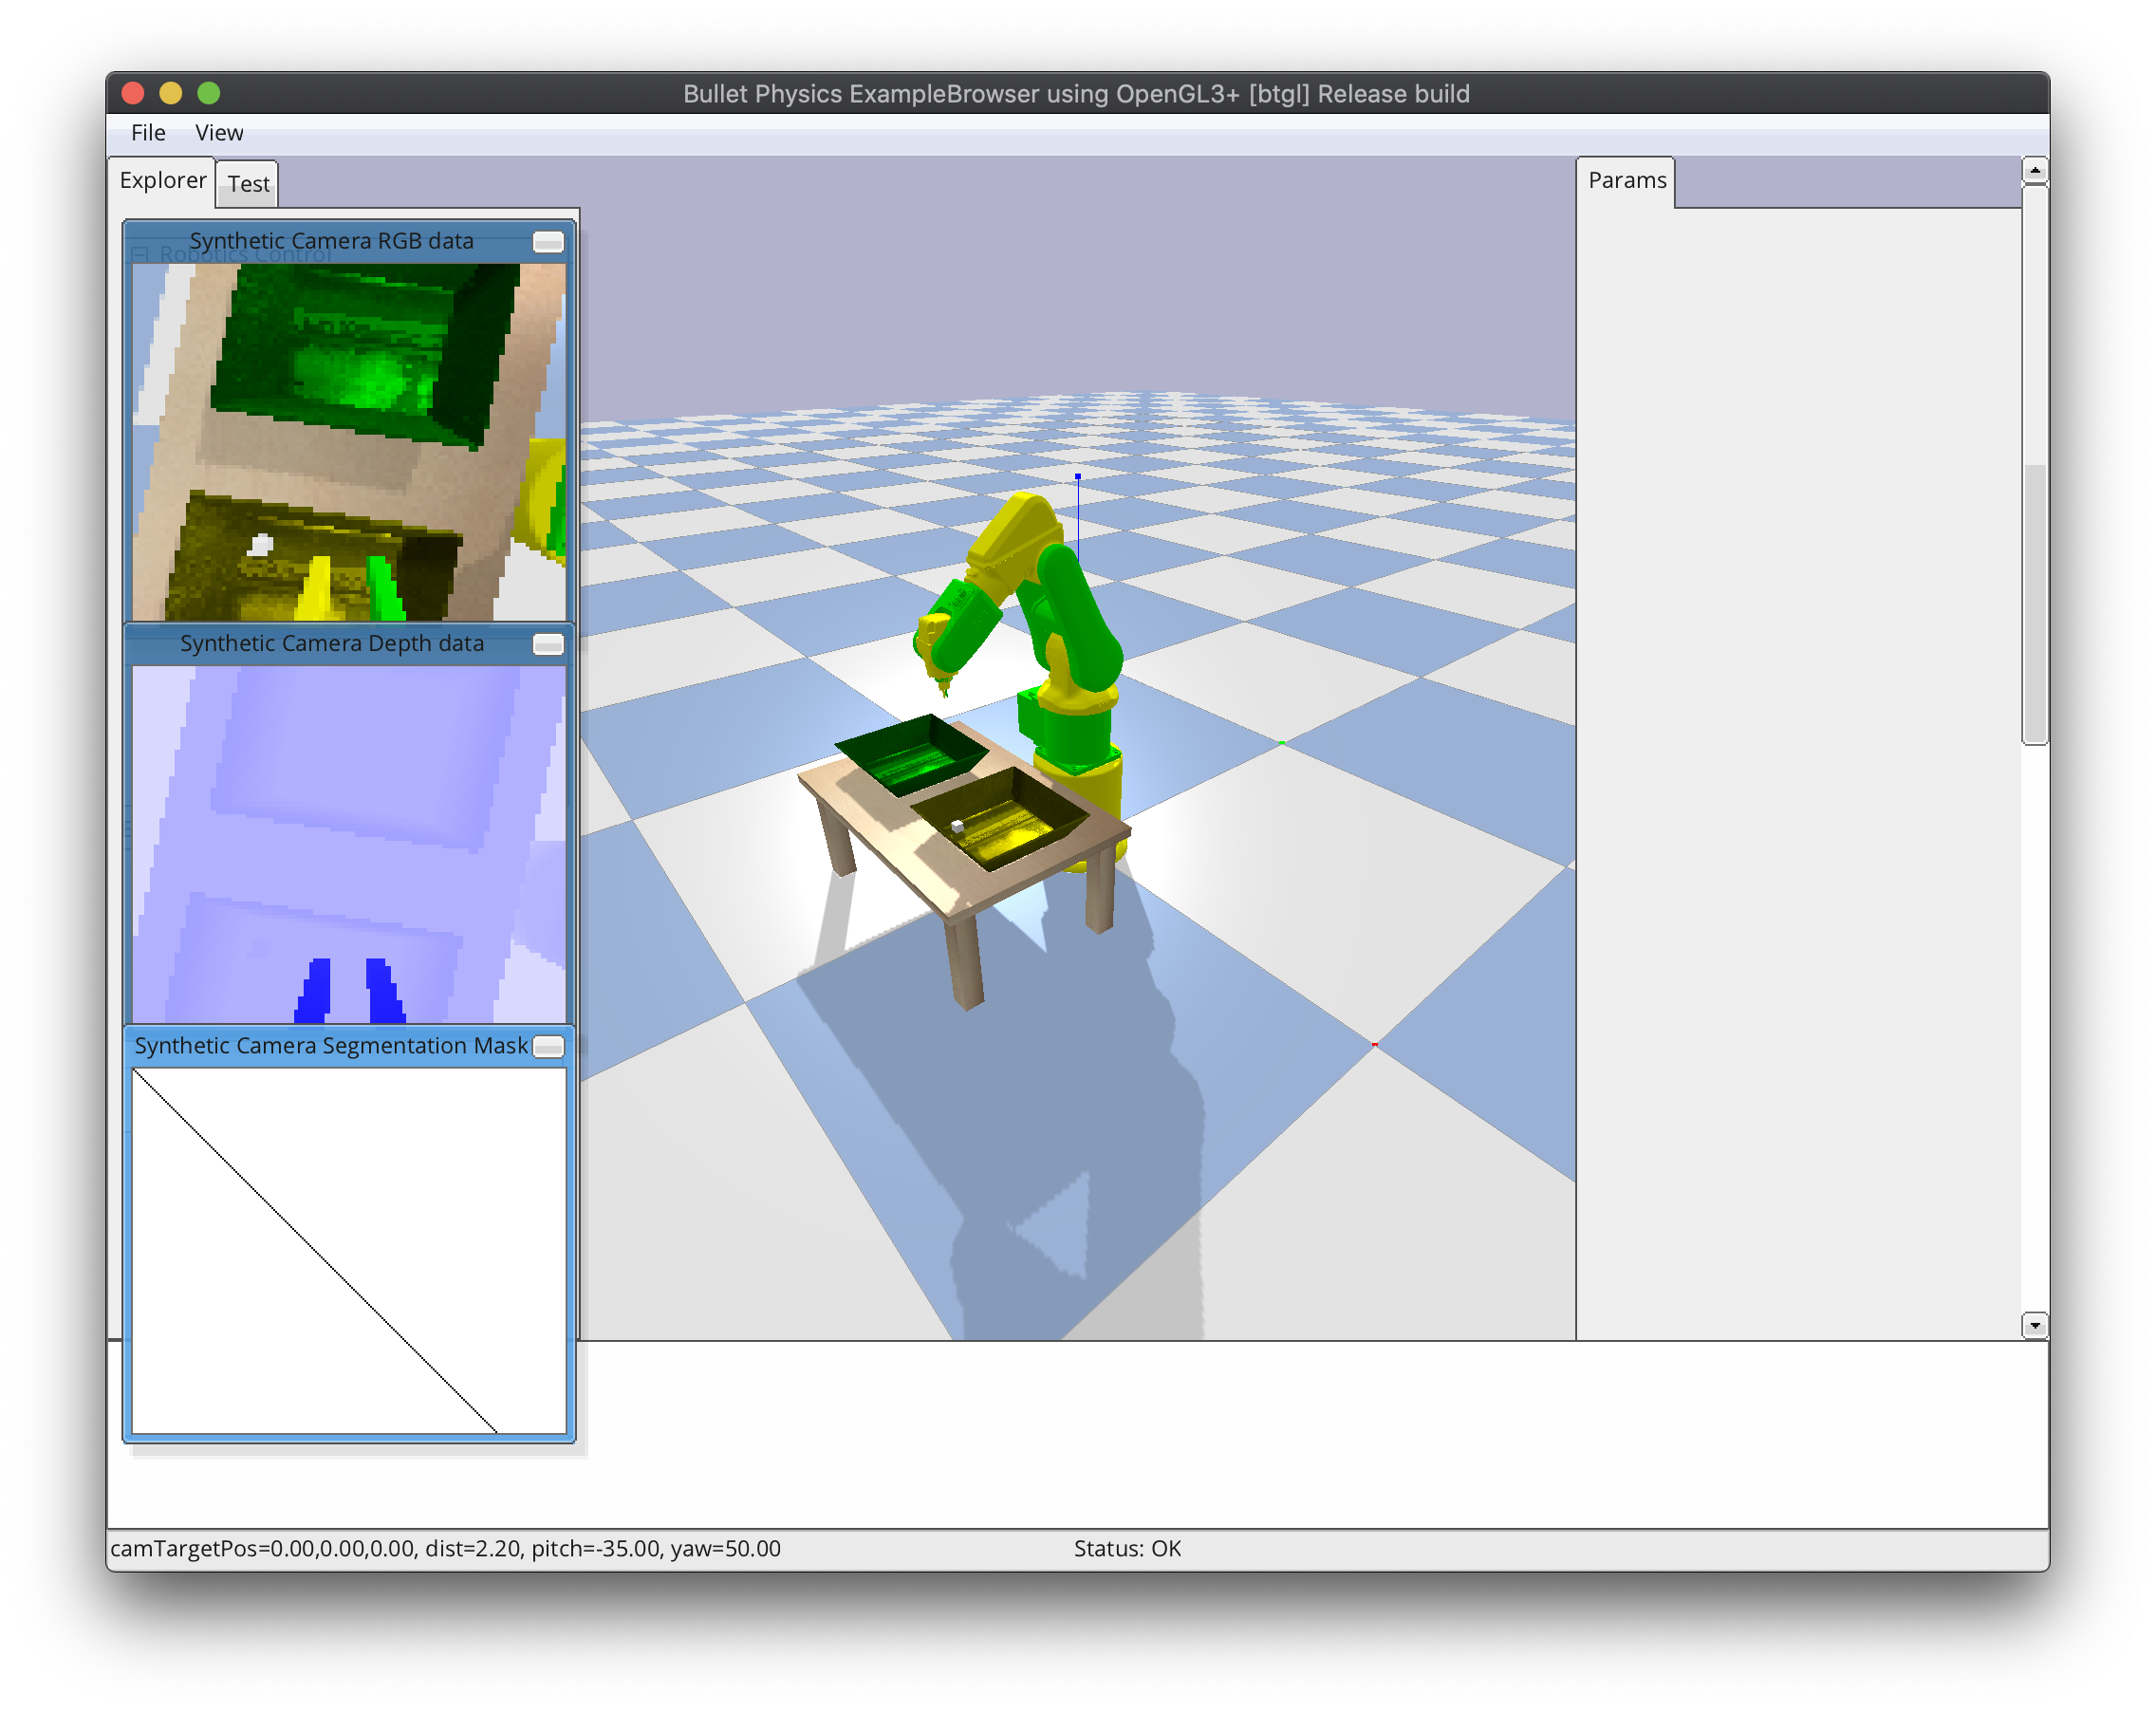
\includegraphics[scale=0.25]{table-clearing-env}
	\caption{Table clearing pybullet environment}
	\label{fig:table-clearing-env}
\end{figure}

\subsubsection{State space}
A RGB-D camera is mounted on the end effector of the gripper. The output of this camera is shown in lFigure \ref{fig:fig:table-clearing-env-camera}. The state space of the environment is a tensor of shape $84 \times 84 \times 4$. The first three channels are RGB pixel values and fourth channel is the depth value.

\begin{figure}[H]
	\centering
	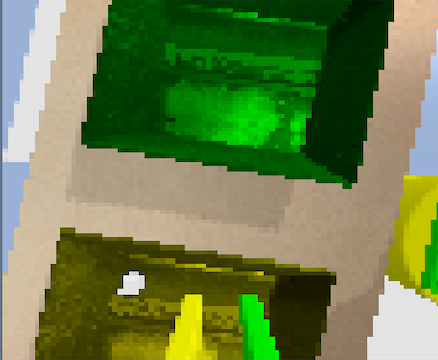
\includegraphics[scale=0.7]{table-clearing-rgb}
	
\includegraphics[scale=0.7]{table-clearing-depth}
	\caption{Gripper camera output; left: RGB, right: depth}
	\label{fig:fig:table-clearing-env-camera}
\end{figure}

\subsubsection{Action space}
\begin{figure}[H]
	\centering
	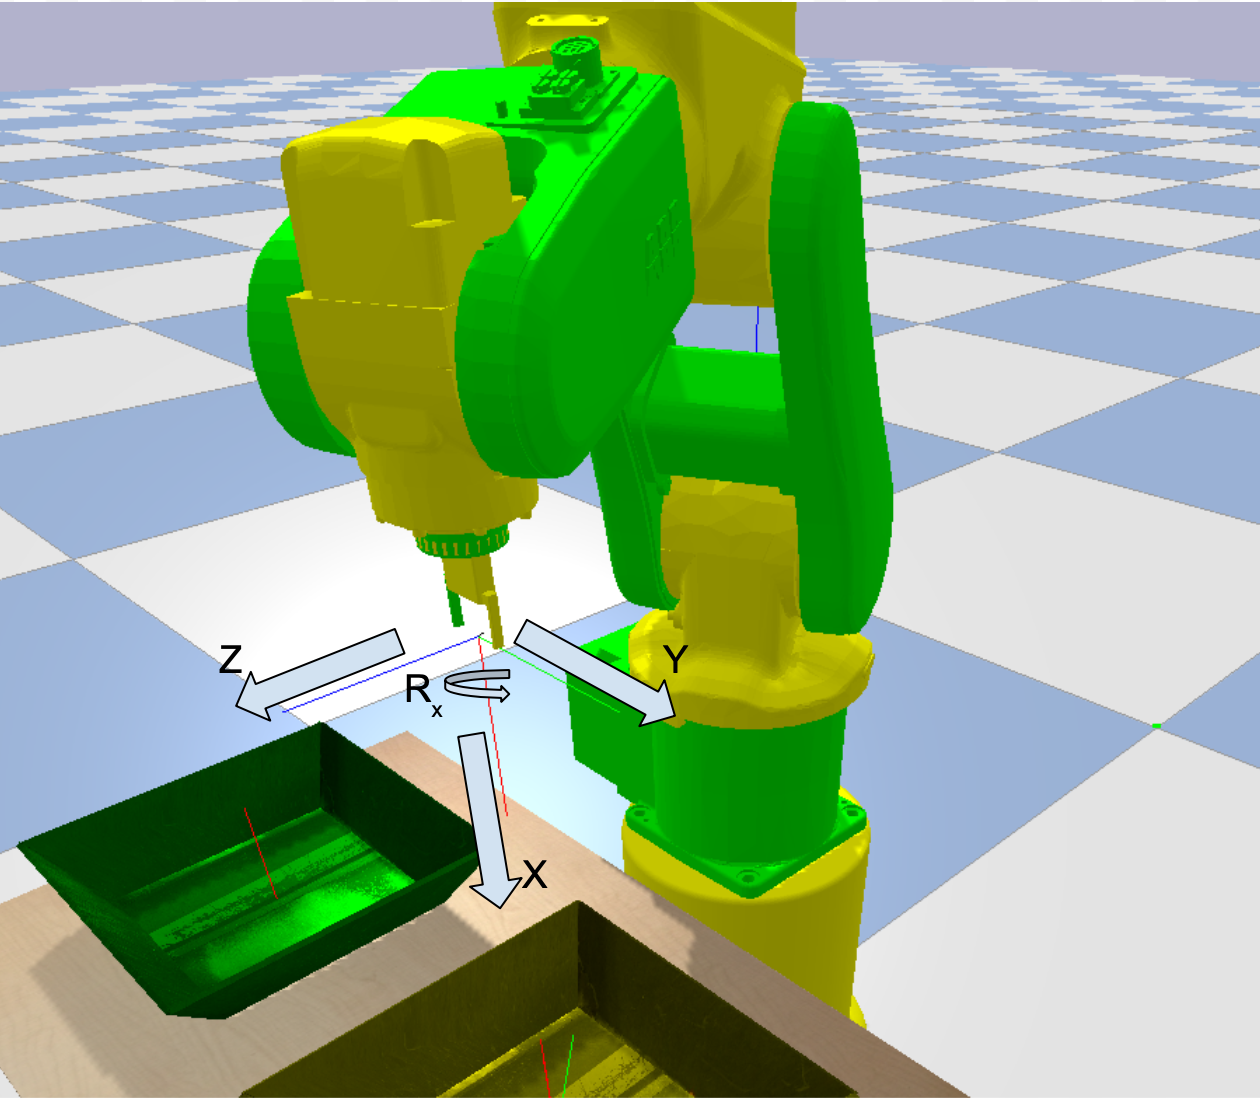
\includegraphics[scale=0.4]{table-clearing-env-action-space}
	\caption{Table clearing environment action coordinate system}
	\label{fig:table-clearing-env-action-space}
\end{figure}

The end effector position can be controlled by making $[\delta x, \delta y, \delta z]$ movements with respect to $X, Y \& Z$  axis of a coordinate system attached to gripper as shown in Figure \ref{fig:table-clearing-env-action-space}. The end effector can be rotated about approach vector by $\delta r_x$. The gripper fingers can be closed by setting binary variable $open$. The maximum/minimum values of a single action is shown in Table \ref{table:table-clearing-env-action-space}

\begin{table}[H]
	\centering
	\begin{tabular}{|c|c|}
		\hline 
		Action & Limit \\ 
		\hline 
		$\delta x, \delta y, \delta z$ & $[-1, 1]$ cm \\ 
		$\delta r_x$ & $[-10, 10] deg$ \\
		$open$ & {1, 0} \\
		\hline 
	\end{tabular}
	\caption{Table clearing environment action space}
	\label{table:table-clearing-env-action-space}
\end{table}

\subsubsection{Reward}
Let $s_t$ and $s_{t-1}$ be environment state at time $t$ and $t-1$ respectively. The total reward returned by the environment for action $a_t$ at time $t$ is the sum of following rewards

\begin{itemize}
	\item If object is not grasped and object has not moved far from initial position and gripper to object distance at time $t$ is less than $t-1$, reward is +1 else -1
	\item If object is grasped and gripper to destination tray distance at time $t$ is less than $t-1$, reward is +1 else -1
	\item For each action, reward of -1 is given to minimize time to complete task
	\item If body of robot including gripper touches any body other than target object, robot is assumed to be collided and a reward of -1000 is given
	\item If at time $t-1$, object is not grasped and at $t$, object is grasped, then a reward of +100 is given. Object is assumed to be grasped when target object is only in contact with gripper fingers and object is having a height of at least 5cm above source tray
	\item If at time $t-1$, object is grasped and at $t$, object is not grasped and target object is not at destination tray, object is assumed to be dropped and a reward of -200 is given
	\item If at time $t-1$, object is not at destination tray and at $t$, object is at destination tray, then object is assumed to be delivered and reward of +200 is given
\end{itemize}

\subsubsection{Episode termination}
A simulation episode is terminated at following conditions
\begin{itemize}
	\item Robot or gripper body is in contact with any body other than target object (collision)
	\item Target object reached destination tray (delivered)
	\item Duration of episode is greater than 3 minutes
	\item Number of actions taken in episode is greater than 3000
\end{itemize}

\section{Hardware specifications}
\subsection{Simulator benchmark}
Simulator benchmark was done on a Lenovo Thinkpad X230 laptop with following specs
\begin{itemize}
	\item Intel(R) Core(TM) i5-3320M CPU @ 2.60GHz processor
	\item 4GB RAM
	\item Integrated graphics
\end{itemize}

\subsection{Testbed evaluation using PPO}
Testbed evaluation using PPO was done on Azure cloud using Standard\_NC12 VM with following specs
\begin{itemize}
	\item Intel(R) Xeon(TM) E5-2690 v3 @ 2.60GHz processor x 12
	\item 112GB RAM
	\item 24GB NVIDIA K80 GPU
\end{itemize}

These VMs are optimized for compute-intensive algorithms like CUDA and OpenCL-based applications and simulations, AI, and Deep Learning. 